\section{Organisation et Méthode}

\begin{frame}
  \begin{block}{Rétrospective}
    \begin{itemize}
      \item Scrum
        \begin{itemize}
          \item Daily \emph{Scrum} (Meeting $\sim$2h30)
          \item \emph{Sprint}
        \end{itemize}
      \item EXtreme Programming
        \begin{itemize}
          \item Pair-programming
          \item Pair-Review + Dir. Technique Review
          \item Roulement des binômes
          \item Convention de code
          \item Refactoring
        \end{itemize}
      \item Itération avec le client
   \end{itemize}
  \end{block}
\end{frame}

\begin{frame}{Scrum}
  \begin{block}{Que reste t-il de Scrum?}
    \begin{enumerate}
      \item Daily meeting concis ($\sim$30 min max)
        \begin{itemize}
          \item Rétrospective de la semaine
          \item (Ré)assignation des taches
        \end{itemize}
      \item \emph{Sprint} soutenu (tous ensemble vers l'objectif)
      \item Communication omni-présente au sein de l'équipe
    \end{enumerate}
  \end{block}
\end{frame}

\begin{frame}{EXtreme Programming}
  \begin{alertblock}{Que reste t-il de XP?}
    \begin{center}
      RIEN
      \begin{figure}
        
\includegraphics[scale=0.7]{img/coding_horror.png}
      \end{figure}
    \end{center}
    \end{alertblock}
\end{frame}


{
\usebackgroundtemplate{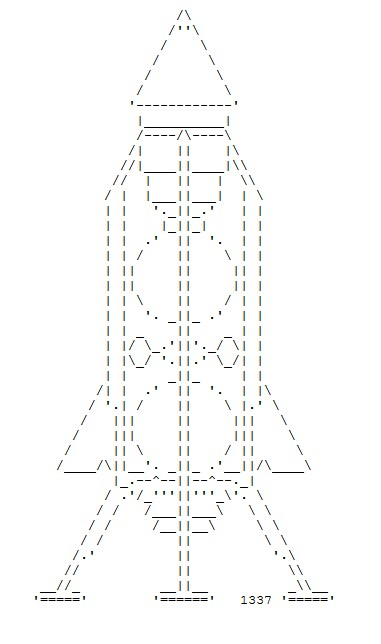
\includegraphics[scale=0.42]{img/rocket.jpg}}%
\begin{frame}{F-Safe Extreme Programming}
  De nouvelle méthode sont apparus suite aux observations des différentes séance de developpement:
  \begin{exampleblock}{FSF-XP}
    \begin{itemize}
    \item (bi|tri)nôme
    \item si un (bi|tri)nôme fonctionne, il se stabilise sinon il y a roulement
    \item review sur retro-projecteur du code avec toute l'équipe
    \item la bulle (avec ou sans fenêtre)
    \item 1 consultant qui consulte les bulles et réponds au questions diverses
    \item deadline plus courte
    \end{itemize}
  \end{exampleblock}
\end{frame}
}

\begin{frame}{Environnement technique}
  \begin{block}{}
    \begin{itemize}
      \item \sout{utilisation de gitHub comme bug tracker}
      \item utilisation de \emph{Lighthouse}: fsafe.lighthouseapp.com (plus simple et clair)
        \begin{itemize}
          \item 3 états: \{open, resolved, hold\}
          \item notifications par email
        \end{itemize}
      \item mise en place de \emph{pre-commit hook}
    \end{itemize}
  \end{block}
\end{frame}

\begin{frame}{Calendrier}
  \begin{itemize}
    \item implémentation (cycle régulier) 
    \item sprint 1, 9/10 Mars
    \item démo client, 12 Mars => \emph{Objectif OK!}
    \item sprint 2, 14/15 Mars
    \item release Candidate 18 Mars => \emph{Objectif OK!}
    \item stabilisation de la Release
    \item livraison, 21 Mars
  \end{itemize}
\end{frame}

\begin{frame}{Déroulement d'un F-Safe day}
  \begin{itemize}
  \item début de séance: On note les taches et les propriétaires au tableau
  \item on definit les taches à réaliser avant manger (\emph{manger blocker})
  \item lorsque un groupe finis une taches, on applaudis et on réassigne
  \end{itemize}
\end{frame}

\begin{frame}{Déroulement d'un F-Safe day}
  \begin{figure}
    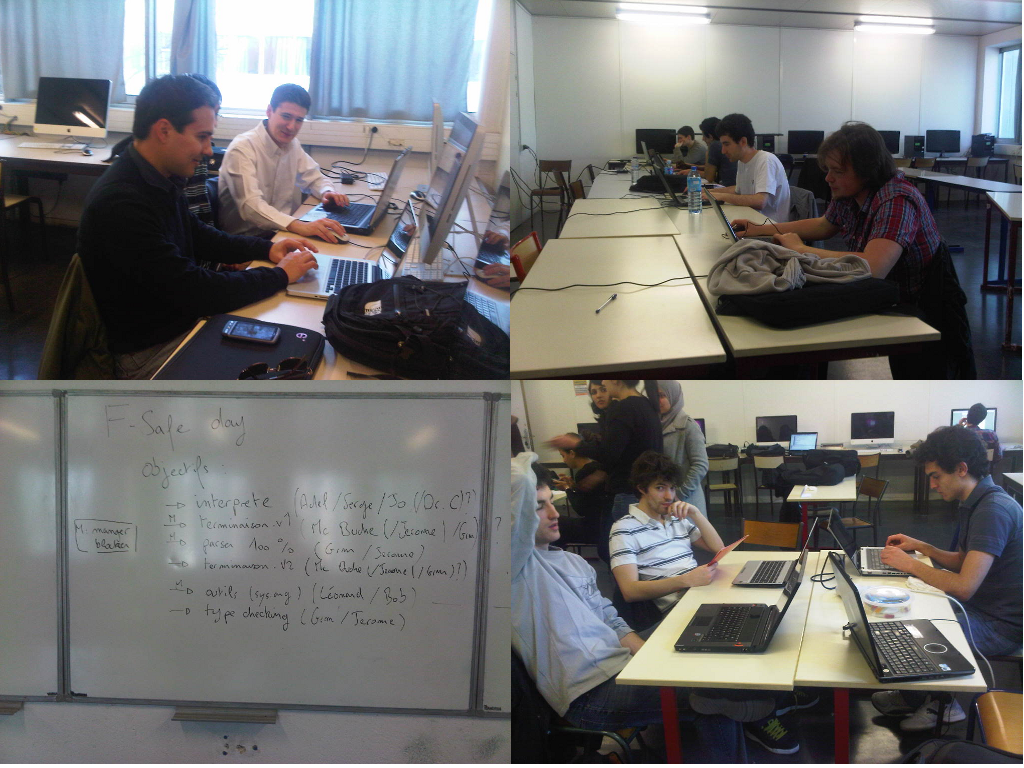
\includegraphics[scale=0.27]{img/FSafeDay.png}
  \end{figure} 
\end{frame}

\begin{frame}{Le travail a distance à 12}
  \begin{block}{}
    \begin{itemize}
      \item Push! Push! Push!
      \item création d'un document de suivi: Task, Status, Comment: \{Owner, Technical Dir.\}
      \item le directeur technique est le seul à fermer la \emph{RC} pour la demo client
    \end{itemize}
  \end{block}

  Laissons-lui la parole...
\end{frame}

